\chapter{Introduction to Beamforming}

\section[Introduction]{\textbf{Introduction}}
In the era of ubiquitous connectivity, wireless communication has become an indispensable aspect of our daily lives. From smartphones to IoT devices, the demand for faster, more reliable, and more efficient wireless networks continues to escalate. To address these challenges, researchers and engineers have turned their attention to beamforming - a transformative technology that revolutionizes wireless communication systems.

\begin{figure}[htb]
\centering
	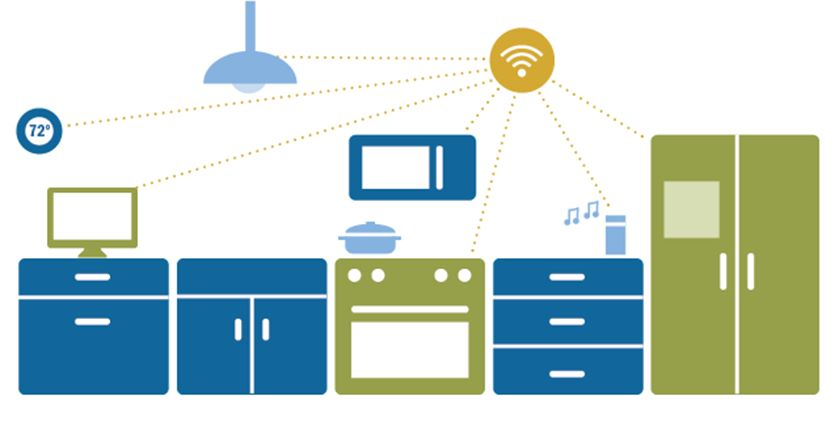
\includegraphics[scale=0.5]{Chapter1/Figures/era}	
	\caption{\label{fig:era}Era of Ubiquitous Connectivity}
\end{figure}

Beamforming is an advanced signal processing technique that enables the focused transmission and reception of electromagnetic waves. By dynamically steering the antenna array's radiation pattern towards specific targets, beamforming offers significant advantages over conventional broadcasting methods. This technology maximizes signal quality, extends coverage range, and enhances network capacity, making it a fundamental area of research and development in the field of wireless communication.

The quest for higher data rates, improved coverage, and enhanced spectral efficiency has led to the emergence of hybrid beamforming techniques. Hybrid beamforming combines the benefits of analog and digital beamforming, offering a promising solution to address the challenges of next-generation wireless networks. To effectively implement hybrid beamforming algorithms, the use of Field-Programmable Gate Arrays (FPGAs) has gained considerable attention due to their flexibility, reconfigurability, and high processing capabilities.

The efficient implementation of hybrid beamforming algorithms necessitates significant computational capabilities, real-time processing, and flexibility to adapt to changing channel conditions. FPGAs provide an ideal platform to address these requirements. Their parallel processing architecture, reconfigurability, and low-latency characteristics make them well-suited for implementing complex digital signal processing tasks, including the extensive matrix operations involved in hybrid beamforming.

\section[Motivation]{\textbf{Motivation}}

As budding engineers of the 21st century, technology is no foreign to us. As a student ourselves, we have at least two if not more smart devices connected to the net at all times. Now with the onset of 5G cellular technology, our expectations wrt data usage has increased even more with ultra fast connectivity becoming a common norm. No doubt our world is progressing in communication technologies and still, we can’t help but wonder why do we still face connection losses while talking on calls! While on a quest to understand the reason behind this, we stumbled upon something called Beamforming and we put our engineering minds to take it upon us and try to improve and explore this major domain of communication engineering! 


\section[Problem statement]{\textbf{Problem statement}}

The design and implementation of a hardware solution for adaptive beamforming pose significant challenges. The problem at hand is to develop a hardware design that effectively adapts to the inbuilt and predefined conditions of the adaptive beamforming, as well as the varying test environments of targets and interferences.

\section[Objectives]{\textbf{Objectives}}
The objectives of the project are
\begin{enumerate}
\item To design and implement a flexible, reconfigurable, and low-latency beamforming algorithm on FPGA.
\item Benchmarking the performance of the implemented design with respect to various parameter constraints such as Speed, Area Utilization and Power consumption and comparing it with the theoretical requirements and other existing beamforming technologies.
\end{enumerate}

\section[Literature Review]{\textbf{Literature Review}}

\textbf{Van Veen et al [1]} classifies beamformers into data independent or statistically optimum, depending on how the weights are chosen. Both are defined with respect to array data where the output of both scenarios are used to optimize the array response. The same procedure is extended to and implemented in spatial filtering.

\textbf{Benesty et al [2]} discusses couple of beamforming techniques by dividing spatial filtering into two parts being synchronization and weight-sum. both methods are discussed with their effects on the beam pattern that is their characteristics of side lobe and main lobe. Beamformers would not yield the same beam pattern for different frequencies and the beam width decreases as the frequency increases.

\textbf{Mucci et al [3]} explains that an input sampling rate Fs, significantly greater than that required for waveform reconstruction, is needed to achieve acceptable approximations to the exact steering delays; frequently, the input sampling rate is five to ten times that required for waveform reconstruction. Interpolation Beamforming  technique is used  for low pass(using zero padding to get higher frequencies) as well as bandpass applications (using Analytic Signal Sampling, Second order Signal Sampling)\\
\textbf{Ulrich et al [7]} explains the need for adaptive array processing in the presence of multiple jammers, conditions for optimal weight computation (SNR), adaptive weight estimation, problems involved in adaptive beamforming,adaptive detection using Maximum Likelihood (ML), Need for Direction of Arrival (DOA)- super resolution.\\
\textbf{Ulrich et al [10]} looks into the grating problem occurring at subarray outputs. s optimization techniques are compared with comparison of resulting grating lobes. The paper concludes that partially overlapping subarrays are the most suited configuration to reduce grating lobes.\\
\textbf{Ulrich et al [11]} defines the advantages of such a design and the analysis. An array containing subarrays is a fairly wide concept that encompasses the situation of steerable directional array elements. At the elements, only phase shifters can also be used to steer all subarrays in a specific direction, and attenuation can be used to control the sidelobe level. The sum of the subarrays then yields the sum beam output. The subarrays may be considered as a super array with components with distinct patterns directed in the desired direction. A completely digital array with Analog to Digital Converters (ADC)s at each antenna element may be ideal, however, it is not practical due to its high weight and cost, resulting in a system with fewer digital receivers.\\
\textbf{Sivasanka et al [5]} explains the effect of the sub array configuration on adaptive beam forming and grating notches in detail with simulation results for ULA. Adaptive beamforming algorithm by using sub arrays, Antenna element and sub-array configurations for simulations has also been shown.\\
\textbf{Zhen-Hai Xu et al [8]} explains how a smart partitioning of a very large planar array into a number of separately fed subarrays offers many interesting design possibilities in antenna synthesis problems. Two typical requirements for the beam scanning - a minimum gain requirement and a sidelobe level requirement - are analyzed whose numerical results illustrate the LFOV technology and validate the analyses.\\
\textbf{Heidelberg et al [1]} decouples Spatial filtering operation into two sub-processes: synchronization and weight-and-sum. The synchronization part controls the steering direction and the weight-and-sum process controls the beamwidth of the main lobe and the characteristics of the sidelobes. Beamformers would not yield the same beam pattern for different frequencies and the beam width decreases as the frequency increases.\\
\textbf{Patel et al [4]} compares Adaptive Beamforming Algorithms LMS, SMI and RLS for ULA Smart Antenna. The radiation pattern achieved by using LMS algorithm is finest. Convergence speed is one the drawback of LMS algorithm as it is directly depends on the step size value. Convergence is low for small value of step size and for large value of step size it becomes unstable. SMI overcomes the limitation of LMS but it increase the complex computation of correlation matrix. RLS algorithm array weights are updates very quickly because the variation of convergence is determined by the knowledge of eigen value of the correlation matrix of signal.\\ 
\textbf{Digdarsini et al [5]} discuss the hardware for digital subsystem consisting of the ADCs, Buffers, FPGA and DAC. The most critical requirement for any DBF system is the reception of the signals from antenna elements at equal phases for baseband processing. This equi-phase clock distribution is achieved by a 1:16 clock distribution card which provides an equi-phase clock for ADCs for sampling signals received from antenna elements.\\
\textbf{Schmidt et al [8]} introduces a novel implementation approach based on SoC technology with optimized Hardware/Software partitioning for real-time delay and sum beamforming. Possible hardware acceleration techniques for beamforming algorithms determining the direction of arrival are analyzed and advantages and disadvantages of the distinct approaches are discussed.\\
\textbf{Raymond et al [16]} introduces new variant of LMS know as the variable step size LMS, where with increase or decrease in mean-square error, the step size increases or lowers, allowing the adaptive filter to follow changes in the system while producing a modest error. The algorithm’s convergence and steady-state characteristics are investigated. The variable step size approach also minimises the misadjustments sensitivity to the level of non stationary conditions.\\
\textbf{Khyati et al [17]} focuses on RLS adaptive algorithm used to compute complex weights. In LMS approach. convergence is slow in an environment giving an array correlation matrix with a large Eigen value spread. The RLS method solves this problem by substituting the gradient step size with a gain matrix. It was observed that increasing the number of antenna array elements results in improved performance.\\ 
\textbf{Arias-García et al [12]} emphasises on an architecture to compute matrix inversions in a hardware reconfigurable FPGA using different floating-point representation precision: single, double and 40-bits. The architectural approach is divided into five principal parts, four modules and one unit, namely Change Row Module, Pivo Module, Matrix Elimination Module, Normalization Module and finally the Gauss-Jordan Control-Circuit Unit. This division allows the work with other smaller arithmetic units that are organized in order to maintain the accuracy of the results without the need to internally normalize and de-normalize the floating point data.\\ 

\section[Brief Methodology of the project]{\textbf{Brief Methodology of the project}}
The main intent of this work is to design and implement  an efficient adaptive beamforming algorithm with FPGA as a traget hardware by making use of Vivado  software as a tool to create an intelligent unit that helps the smart antenna system to understand about the  signal of interest and the jamming signals and respond accordingly. The figure \ref{fig:methodology} explains in detailed steps about how to choose a required algorithm to achieve required results,how to proceed for design of the same using a hardware descriptive language for implementation and how to assure and evaluate the design performance.The evaluation of the HDL results are verified using the the Matlab results to define the accuracy of the system and performance of the final system is defined on the speed, accuracy,power and area utilization.
\begin{figure}[h]
\centering
	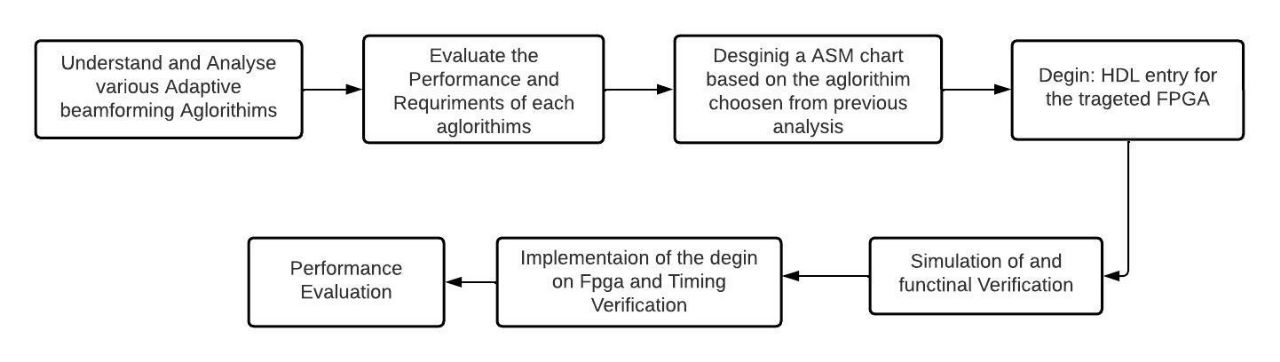
\includegraphics[scale=0.5]{Chapter1/Figures/methodology}	
	\caption{Flow of Work}
	\label{fig:era}
\end{figure}

\section[Assumptions made / Constraints of the project]{\textbf{Assumptions made / Constraints of the project}}
The following assumptions are made while carrying out the work:

\begin{enumerate}
\item Information about grouping of antenna elements into sub array which can be regular or irregular \item Presence of a digital signal processor is assumed which is used as a communication interface between the targeted hardware and the antenna system
\item The implememted algorithm is designed to work with all sizes of inputs and its capability is limited only by the targeted hardware specifications such as the number of LUTs in the FPGA (minimum 3,00,000)
\end{enumerate}

\section[Organization of the report]{\textbf{Organization of the report}}

This report is organized as follows:

\begin{itemize}
\item Chapter 2 discusses the fundamentals of array processing, needs and types of beamforming and the signal models
\item Chapter 3 discusses about the types of algorithms which are suitable for the design of adaptive beamforming and their comparison.   
\item Chapter 4 briefly describes the methodology of the desgin and implementation of the SMI algorithm in Vivado software and optimization technique used to achieve the final design
\item Chapter 5 illustrates the results of the implementated design and comments on the performance of the desgin
\item Chapter 6 tells about the improvisation(s) that can be done and the future scope of the current design
\end{itemize}

.